\section{Motivation} \label{motivation-l}
DNA methylation is a well studied chemical modification of DNA, which occurs when a methyl group is attached to a DNA nucleotide. It is associated with diverse biological processes of direct clinical relevance, including gene and transposon silencing, X-chromosome inactivation, and  genomic imprinting \citep{Li1993, Mohandas1981}. In mammals,  methylation is observed almost exclusively on cytosine residues in the context of CpG dinucleotides (\ie C followed by G, where p stands for the phosphate group linking C and G). DNA methylation is said to be a true \emph{epigenetic modification}, since its mechanism of inheritance during the cell cycle is well established \citep{Law2010}. 

Due to the increased vulnerability of the 5-methylcytosines to randomly deaminate to thymine, most of the genome is depleted from CpG dinucleotides \citep{Scarano1967}, except from small regions termed \emph{CpG islands} \citep{Bird2002}. A CpG island (CGI) is a sequence of at least 200 bp with a greater number of CpG sites than expected from its GC content. These regions are often GC rich, typically undermethylated, and are found upstream of many mammalian genes \citep{Law2010}. 

Bisulphite treatment \citep{Frommer1992} followed by next generation sequencing (NGS) can be used to measure the methylation level of the genomic DNA at a single-nucleotide resolution, and is termed Whole-Genome Bisulphite Sequencing (WGBS). Sodium bisulphite efficiently deaminates unmethylated cytosines to uracils and leaves the 5-Methylcytosines unchanged. During sequencing, unmethylated cytosines are read out as thymines. Reads are then aligned to a reference genome allowing changes of C to T during the mapping procedure. 

The outline of the bisulphite treatment of a sample DNA sequence is shown in \emph{Figure \ref{bisulphite-pic}}.

\begin{figure}[!h]
	\begin{center}
 		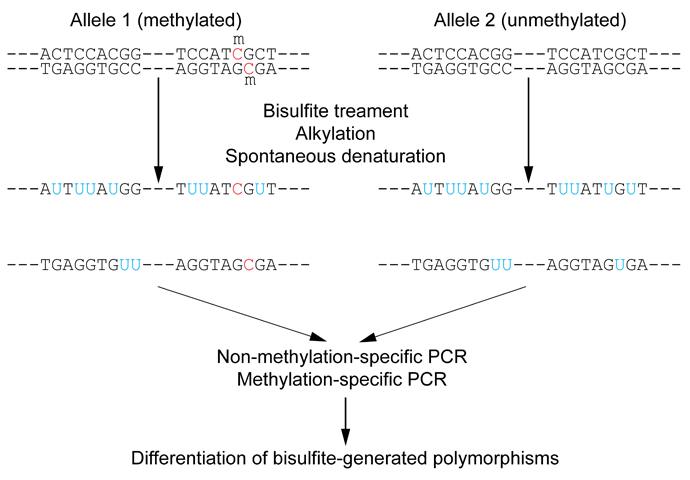
\includegraphics[scale = 4]{images/bisulphite.png}
		\caption{\emph{Outline of the bisulphite treatment of a sample DNA sequence. Unmethylated cytosines are deaminated to uracils by bisulphite and are shown in blue, while 5-Methylcytosines are resistant to conversion and are shown in red.}}
		\label{bisulphite-pic}
	\end{center}
\end{figure} 

In WGBS experiments, the DNA molecules often originate from distinct cells, as a consequence, the methylation state of a particular cytosine may be different across DNA molecules. Hence, in the context of WGBS experiments the methylation of a particular cytosine is described as \emph{methylation level}, which is the fraction of the molecules in the sample containing 5-Methylcytosine at the specific genomic locus \citep{Schultz2012}. \emph{Read coverage} is the average number of times a CpG site is read during the sequencing process, and this depends on the depth of the sequencing.

\cite{Meissner2005} developed a technique, termed Reduced Representation Bisulfite Sequencing (RRBS), for analyzing the genome-wide methylation profiles efficiently, at lower cost and with greater coverage of CpG dense regions. This method, combines bisulphite treatment and restriction enzymes, such as MspI, to generate a 'reduced representation' of the genome of a strain, tissue or cell type which have a high CpG content \citep{Meissner2005}. 

What is often of practical interest is identifying the methylation profile of a genomic region, \eg the methylation profile of a promoter. \cite{Vanderkraats2013} suggested that the shape of the methylation profile plays an important role in predicting gene expression, leading to a potentially functional role for methylation patterns. This means that higher-order properties, such as shape, of the methylation profiles over a region should be considered. Taking into consideration that the methylation level of a CpG site is highly correlated with the methylation level of the surrounding CpGs (\ie spatial co-dependence), \cite{Mayo2014} developed M$^3$D, which is non-parametric kernel-based method for statistical identification of differentially methylated regions (DMRs). This project makes the same assumption about the \emph{spatial co-dependence} of CpGs, but is mainly concentrated in clustering together similar methylation profiles.

\section{Modelling DNA methylation profiles}
DNA methylation data generated from next generation sequencing methods can be modelled with a Binomial distribution. Assume that \emph{t} is the total number of reads that are mapped to a specific CpG site, and that the 5-Methylcytosine were found in \emph{m} of these reads. Then for each CpG cite we have the read proportion \emph{(m,t)}, and we assume that:

\begin{equation} \label{binom-1d-f}
	m \sim Binom(t, p)
\end{equation}

where \emph{p} is the unknown methylation level of the CpG site.

We are interested in modelling methylation profiles across different genomic regions, \eg promoter regions, hence the data can be represented as a set of vectors, whose dimensionality \emph{L} depends on the number of the individual CpG sites for that specific region. Thus, each region \emph{i} can be represented by a vector $\mathbf{y}_{i}$ of dimensionality $L_{i}$, and each entry of the vector consists of the tuple:

\begin{equation}
	%n_{i}^{l} = \frac{m_{i}^{l}}{t_{i}^{l}}
	y_{il} = (m_{il},t_{il})
\end{equation}

where, $m_{il}$ is the number of 5-Methylcytosine reads on $l$-th CpG site in region $i$, and $t_{il}$ is the total number of reads on $l$-th CpG site in region $i$. Thus, 

A promising approach for modelling the methylation profile for a given region is to use a \emph{Gaussian Process} for classification \citep{Rasmussen2006}. Even though this approach would be ideal, its time complexity of $O(n^{3})$ is prohibitive for our problem. Thus, we have to resort in modelling the methylation level using $n^{th}$ degree polynomial functions.

More specifically, let $\mathbf{x}_{i}$ be the genomic region of interest, $\mathbf{y}_{i}$ be the observations in this region (\ie proportions of methylated reads to the total reads at each site), and let $f(\mathbf{x}_{i})$ be a latent function representing the methylation profile at that specific genomic region. Since the methylation data take values in the $[0, 1]$ interval, we introduce a latent function $g(\mathbf{x}_{i})$, \eg $g(\mathbf{x}_{i}) = \alpha \mathbf{x}_{i}^{2} + \beta \mathbf{x}_{i} + c$, defined as the \emph{inverse probit transformation} of $f(\mathbf{x}_{i})$. In other words, $f(\mathbf{x}_{i})$ is the probit transformation of $g(\mathbf{x}_{i})$:

\begin{equation} \label{probit-transform-f}
	f(\mathbf{x}_{i}) = \Phi(g(\mathbf{x}_{i}))
\end{equation}

where $\Phi(x)$ is the Cumulative Distribution Function (CDF) of the standard normal distribution:

\begin{equation} \label{cdf-stand-normal-f}
	\Phi(x) = \frac{1}{\sqrt{2\pi}} \int_{-\infty}^{x} e^{-t^{2}/2}dt
\end{equation}

Let $\mathbf{f}_{i} = f(\mathbf{x}_{i})$ and $\mathbf{g}_{i} = g(\mathbf{x}_{i})$ be shorthand for the values of the latent functions.

Given the values of the latent function $\mathbf{f}_{i}$, the observations at each CpG site for that region are independent Binomial variables, as shown in \emph{Eq. \ref{binom-1d-f}}, so the joint likelihood factorizes and we have:

\begin{equation} \label{likel-binom-prob-f}
  \begin{split}
	p(\mathbf{y}_{i}|\mathbf{f}_{i}) & = \prod_{l=1}^{L} p(y_{il}|f_{il}) \\
							 & = \prod_{l=1}^{L} Binom(t_{il}, f_{il}) \\
							 & = \prod_{l=1}^{L} Binom\big(t_{il}, \Phi(g_{il})\big) \\
							 & = \prod_{l=1}^{L} \binom{t_{il}}{m_{il}} \Phi(g_{il})^{m_{il}} (1 - \Phi(g_{il})\big)^{t_{il} - m_{il}}
  \end{split}
\end{equation}

In practice, the likelihood is computed in the log space, due to numerical issues when multiplying many probabilities of small numbers leading to underflow errors. Thus, the joint log likelihood is:

\begin{equation} \label{likel-binom-prob-f}
  \begin{split}
	\log p(\mathbf{y}_{i}|\mathbf{f}_{i}) & = \sum_{l=1}^{L} \log p(y_{il}|f_{il}) \\
				& = \sum_{l=1}^{L} \log \bigg(\binom{t_{il}}{m_{il}} \Phi(g_{il})^{m_{il}} \big(1 - \Phi(g_{il})\big)^{t_{il} - m_{il}}\bigg) \\
				& = \sum_{l=1}^{L} \bigg(\log \binom{t_{il}}{m_{il}} + m_{il} \log \Phi(g_{il}) + \big(t_{il} - m_{il} \big) \big(1 - \Phi(g_{il})\big)\bigg)
  \end{split}
\end{equation}